% Bagian Tugas Pendahuluan
\section*{Tugas Pendahuluan}
\begin{enumerate}
  \item Jelaskan bagaimana cara kontrol 7-segment anoda dan katoda? \\
Cara mengontrol 7-segment anoda adalah dengan menerapkan sinyal rendah ke katodanya. karena semua anoda dijadikan 1 pin yang sama kemudian dihubungkan ke tegangan suplai positif.\\\\
Cara mengontrol 7-Segment katoda adalah dengan mengalirkan tegangan positif ke terminal anodanya. Karena semua katoda pada 7-segment dihubungkan bersama ke satu pin umum, dan pin ini biasanya dihubungkan ke ground.\\
  \item Buat schematic di Tinkercad untuk menampilkan nomor kelompok menggunakan
dua 7-segment! \\
\end{enumerate}
  \begin{figure}[H]
\centering
% Kalau mau menambah gambar lagi tinggal nambahin begin{subfigure} -> end{subfigure}
  \begin{subfigure}[b]{0.4\linewidth}
    \centering
    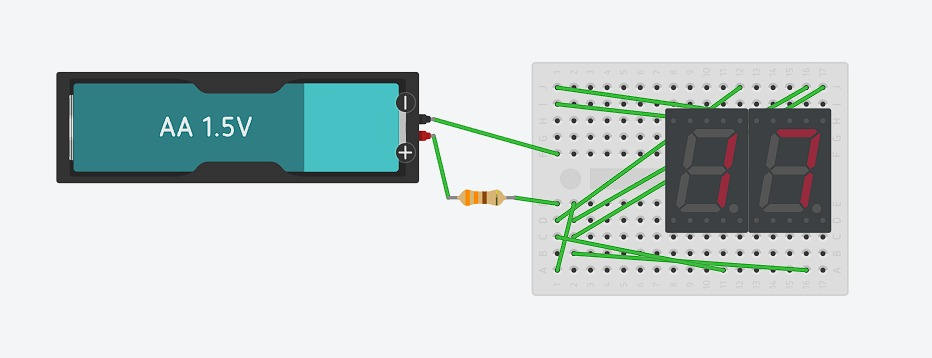
\includegraphics[width=\linewidth]{img/circuit.jpeg}
    \caption{Gambar circuit untuk menampilkan nomor 17.
    \label{fig:inisub1}}
  \end{subfigure}
\hspace{1cm}
  \begin{subfigure}[b]{0.4\linewidth}
    \centering
    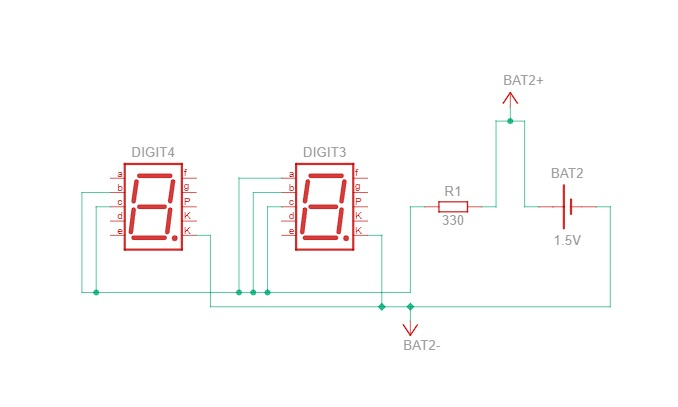
\includegraphics[width=\linewidth]{img/schema.jpeg}
    \caption{Gambar schema untuk menampilkan nomor 17.
    \label{fig:inisub2}}
  \end{subfigure}
  \caption{Gambar untuk jawaban soal pendahuluan 2.
  \label{fig:keduagambar}}
\end{figure}